\documentclass{article}
\usepackage{graphicx} % Required for inserting images
\usepackage{amsmath}
\usepackage{esvect}
\usepackage{booktabs}
\usepackage{float}
\usepackage{enumerate}
\usepackage{hyperref}

\title{\textbf{Secure Multi-Party Computation
}Assignment 4 - BeDOZa protocol, active (malicious) adversary\textbf{}}
\author{Or Dinar \\
        Liad Ackerman \\
        Maayan Ben Zion}
\date{26.02.2024}

\begin{document}

\maketitle

\section{BeDOZa - Theory}

In this assignment we enhance our implementation of BeDOZa protocol (assignments 3) to
achieve security against malicious adversaries (security with abort), Using MACs to authenticate secret shares, as shown in class.
\newline

Reminder:
\paragraph{Equation 3:}

$$
f_{\overrightarrow{a},4}(x_{1},x_{2})=\begin{cases}
			1 & \text{if $a_1x_1 + a_2x_2 \geq 4$ }\\
            0 & \text{otherwise}
		 \end{cases} \hspace{1cm} for \hspace{.25cm}  \overrightarrow{a} \in {\left\{ 0,1,2,3\right\}}^{2}
$$



\subsection{What does it do?}
We recall that BeDOZA protocol uses the idea of \textit{Secret Sharing Schemes} in order to securely compute an operation of a logical gate. In boolean circuits, It does this by picking a random bit $r$ and computing $r \bigoplus x$ where $x$ is an input bit. \newline
In boolean circuits Secret Sharing Schemes have the following functions:
\begin{itemize}
  \item Shr($x$) - provided an $x$, pick a random bit (0 or 1) $r$ and return ($r$, $r \bigoplus x$).
  \item Rec($S_1,S_2$) - reconstructs the secret input buy applying $\bigoplus$ between the secret sharing themselves, then computing the XOR between the products.
  \item OpenTo(P,$S_1$) - returns $r\bigoplus r \bigoplus x$ to the party P, which, in turn, is the secret $x$.
  \item Open($S_1$) - returns $r\bigoplus r \bigoplus x$ to all parties.
\end{itemize}
\newpage


\subsection{Implementation}
In addition to previous functions shown in \textit{Assignment 3}, we also implemented the necessary functions to achieve Message Authentication Code (MAC) in order to further enhance our protocol.The added functions in the python implementation are the following:

\begin{itemize}
  \item gen(): 
  Generates a random pair $k=(r,n)$ $\in$ ${Z_2}^{2}$
  \item tag(k,x): Returns $r*m+n$ where $(r,n)=k$ is a generated random pair, and $m$ is a message
  \item ver(tag,k,x): verifies that $tag$ is indeed $r*m+n$ where $tag$ is a given value calculated using a tag() function, $(r,m)=k$ is a generated random pair, and $m$ is a message
  \item check(bool): aborts the program in case ver() fails

\end{itemize}

\textbf{Note:} In the previous assignment we implemented the AND functions such that each gate receives two secret shares and returns a secret share. Thus, we concluded that the only option for a malicious adversary to manipulate the data is by changing the first layer of inputs in the Boolean Circuit. As seen in Figure 1 below - these input gates corresponds to the first 8 AND gates.

  
\section{Equation 3's Boolean Circuit}
We'll provide an image of the boolean circuit for Equation 3 for reference.
\begin{figure}[H]
    \centering
    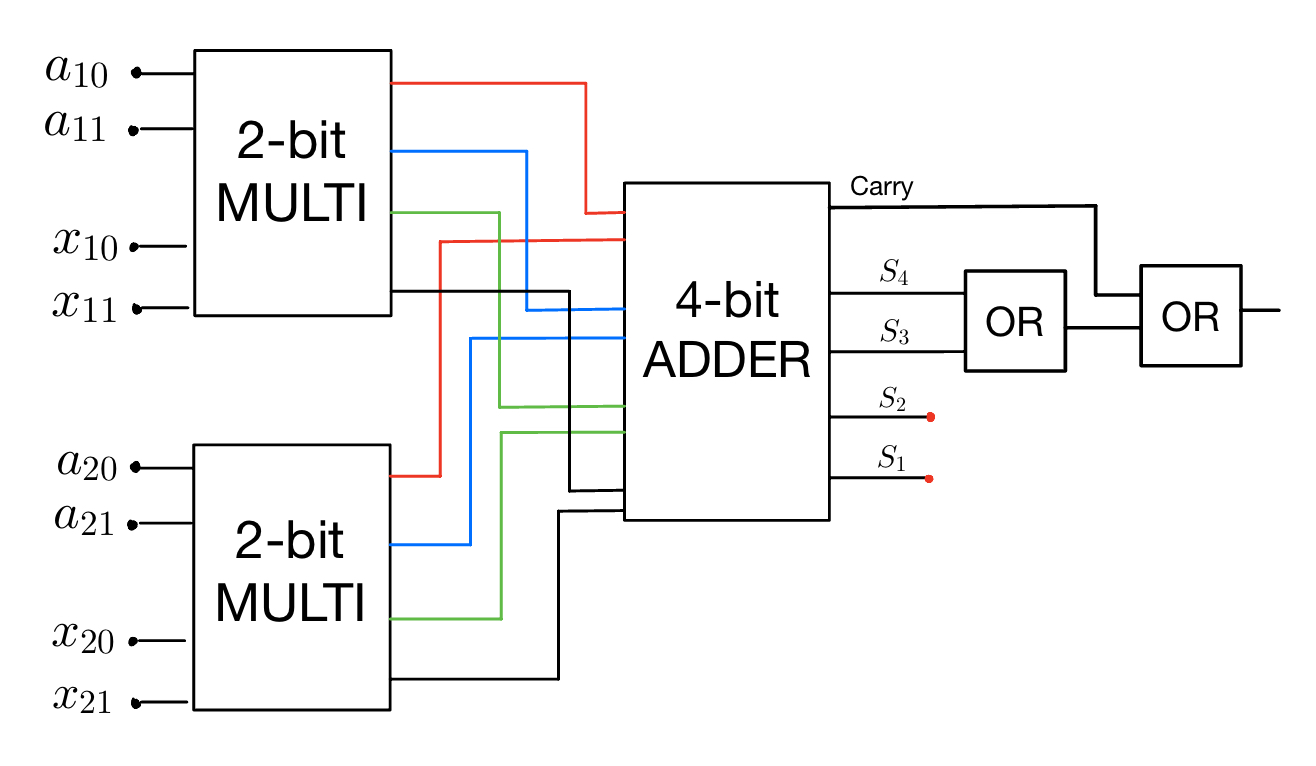
\includegraphics[width=1\linewidth]{FinalBooleanCircuit.jpeg}
    \caption{Boolean circuit that represents $Equation$ $3$.}
    \label{fig:enter-label}
\end{figure}

\newpage

\subsection{Using the functions}

We begin by dividing each bit of Alice's input and Bob's input such that Alice receives the first bit of each bit's secret share and Bob receives the second. Then, by calling \textit{gen()} function 8 times, we generate 8 random pairs $(r,n)$ (one for every AND gate). We then calculate Alice's tags for her shares from her input $a$ and from Bob's input $x$, using the \textit{tag()} function. Similarly, Bob does the same with his shares. Then, for each of the first 8 AND gates, we check that the tag that was calculated with the gate corresponding expected input wires, is indeed the same as the tag calculated using the actual gate's input wires, by calling the \textit{ver()} function. 

\textbf{Note:} We implemented a one sided MAC where Alice checks for changes in Bob's inputs. Symmetrically, we can implement this protocol such that Bob checks for changes in Alice's input, and also for both of them to check.

\section{In Conclusion}
We enhanced our implementation of BeDoZa protocol using MAC as shown in class. By that we achieved a secure way to compute the given equation and defending against a malicious adversary.

\end{document}
